% XeLaTeX can use any Mac OS X font. See the setromanfont command below.
% Input to XeLaTeX is full Unicode, so Unicode characters can be typed directly into the source.

% The next lines tell TeXShop to typeset with xelatex, and to open and save the source with Unicode encoding.

%!TEX TS-program = xelatex
%!TEX encoding = UTF-8 Unicode

\documentclass[11pt]{article}


%%%%%%%%%%%%%%%
\def\Type{ApplicationDJ}
\def\TypeNum{During-class for Application Day: Gradient Descent Method}
\def\TypeTitle{}
\def\Semester{Fall 2025}
\def\Course{Math 1190/1210}
\def\Targets{{\bf\color{Goldenrod}AD1}}
\def\pTableCellNum{9}
\def\learningRateCellNum{8}
\def\mbTableCellNum{11}
\def\exNum{$3$} %This exists because \label{} is not picking up $3$ from Example 3. Change if example ordering changes



\usepackage{preambleDJ}
\usepackage{footnote}
\makesavenoteenv{minipage}



\begin{document}
\pagestyle{otherpages}
\thispagestyle{firstpage}
\vspace*{.65in}

%If Ada Lovelace\footnote{\url{https://en.wikipedia.org/wiki/Ada_Lovelace}} is the ``mother of programming" then 
{\bf Introduction}\\
Fei-Fei Li is  known as the ``godmother of A.I" for her  groundbreaking contributions in computer vision and deep learning and as the creator of ImageNet\footnote{
See ``Godmother of A.I." Fei-Fei Li on technology development: ``The power lies within people" at \url{https://www.cbsnews.com/news/godmother-of-a-i-on-technology-development-fei-fei-li/}\\
 or Britannica at \url{https://www.britannica.com/biography/Fei-Fei-Li}, The Guardian \href{https://www.theguardian.com/technology/2023/nov/05/ai-pioneer-fei-fei-li-im-more-concerned-about- the-risks-that-are-here-and-now}{\underline{here}} or \url{https://en.wikipedia.org/wiki/Fei-Fei_Li} }. 
~\\\\
\mpageT{.35}{.65}{
%\graphicsR{adaLovelace2}{2}
\graphicsL{feiFeiLiWiredCropped}{2}
}
{
In this application, we will be exploring how the tools of calculus can be applied in machine learning. \textit{Machine learning} refers to computer programs for which the outputs mimic patterns in a specific dataset, but without these patterns being explicitly described in the programming. This field powers much of modern artificial intelligence. For example, while generative AI's like ChatGPT can produce coherent English sentences, their code does not contain the rules of English grammar and syntax; rather, they ``learn" these rules autonomously by processing large amounts of examples. \\\\
%
This learning process can be viewed as an optimization problem in the following way:
\begin{itemize}
    \item The algorithm to generate new outputs contains many \textit{parameters,} which each influence the outputs generated.
    \item Once the parameters have been chosen, the outputs of the algorithm are compared against the data set. The algorithm is then given a \textit{loss} score, where a smaller loss indicates a closer match to the data.
    \item The \textit{loss function} takes the parameters as input and gives the loss of the corresponding algorithm as an output. The optimization problem is then to find the parameter set which minimizes the loss function.
\end{itemize}
}~\\

Unfortunately, this optimization problem is usually much harder than the ones we've seen in this class so far. One big difference is the number of inputs: every function we've seen has had just one input $x$, while machine learning models can have billions of parameters or more. This means it is very hard to visualize or graph the loss function. Another issue is that the function itself is so complicated that we cannot simply write down the derivative and find critical numbers in the usual way.

In this situation, one of the tools we can use is \textit{gradient descent}. Gradient descent is a method used for optimization which only requires us to be able to evaluate a function and its derivative at individual points in the domain. Throughout this worksheet, we will develop the ideas of gradient descent for a single-variable function $f(x)$.
\newpage
{\bf Example 1: Function and Derivative}\\

Suppose that we evaluate our function and its derivative at $x=1$ to get that $f(1) = 1$ and $f'(1) = 2$.

\begin{enumerate}
\item Find the equation of the line tangent to $f(x)$ at the point $(1,1)$:\vs{.5}
\[
    y = \unlineb{2}{}
\]
\end{enumerate}

A small segment of the tangent line is sketched below in red, along with an example in blue of what $f(x)$ might look like near the point $(1,1)$.

\begin{center}
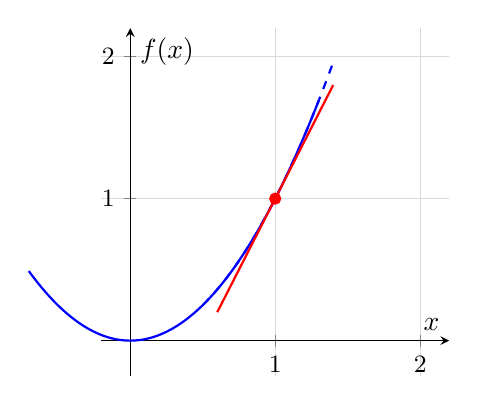
\begin{tikzpicture}
\begin{axis}[
    height = 6cm,
    width = 6cm,
    axis lines=middle,
    xlabel=$x$, ylabel=$f(x)$,
    xmin=-0.2, xmax=2.2,
    ymin=-0.25, ymax=2.2,
    xtick={0,1,2},
    ytick={0,1,2},
    grid=both,              % add grid lines
    grid style={gray!30},   % light gray grid
    tick label style={font=\small}, % smaller labels
    enlargelimits=false,
    clip=false
]

% f(x) = x^2
\addplot [domain=-0.7:1.3, samples=100, blue, thick] {x^2};
\addplot [domain=0.5:1.4, samples=100, blue, thick, dashed] {x^2};

% Tangent at x=3: f'(3) = 6
\addplot [domain=0.6:1.4, red, thick] {2*(x-1)+1};

% Mark the point (3,9)
\addplot[only marks, mark=*, red] coordinates {(1,1)};
% \node[below right] at (axis cs:1,1) {$(1,1)$};

\end{axis}
\end{tikzpicture}
\end{center}

Call the $x$-value we're currently examining $x_1=1$. We want to choose a new guess $x_2$ which is closer to the minimum of $f(x)$.
From this picture, we can see that since $f'(x_1)>0$, if we pick $x_2 < x_1$ then hopefully  $f(x_2)$ is closer to the minimum. But how much smaller should we make $x_2$? If we change our guess too much, we may overshoot the minimum, but if we change it too little we won't make much progress towards finding the minimum. 

The formula we will use to update our guess is this:
\[
    x_2 = x_1 - \alpha f'(x_1),
\]
where $\alpha$ is some positive constant.
\begin{enumerate}
    \item[2.]  Using $\alpha = 0.1$, compute $x_2$ in our example.\vs{1.5}
    \[
        x_2 = \unlineb{2}{}
    \]
\end{enumerate}
\newpage
This formula makes sense because:
\begin{itemize}
    \item If $f'(x_0)>0$, this moves our guess to the left, just like we wanted. If $f'(x_0) < 0$, this moves our guess to the right.
    \item If $f'(x_0)$ is close to zero, then we're probably close to the minimum and our guess won't move much. If $f'(x_0)$ is large, then the guess will change significantly.
    \item Adjusting the constant $\alpha$ allows us to fine-tune the gradient descent process, either speeding it up or making sure we don't overshoot the minimum.
\end{itemize}
We can then use $f'(x_2)$ to make a new guess $x_3$, use $f'(x_3)$ to make a new guess $x_4$, and so on and so forth until we are confident our guess is close to the minimum.
\begin{figure}[h!]
\centering
\begin{minipage}{0.45\textwidth}
\centering
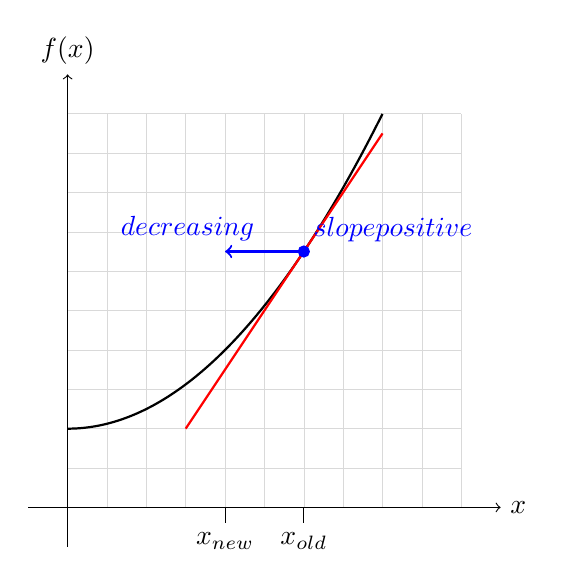
\begin{tikzpicture}[scale=1.0]
    % grid
    \draw[step=0.5, gray!30, very thin] (0,0) grid (5,5);
    
    % axes
    \draw[->] (-0.5,0) -- (5.5,0) node[right] {$x$};
    \draw[->] (0,-0.5) -- (0,5.5) node[above] {$f(x)$};
    
    % function
    \draw[thick, domain=0:4, samples=100, smooth] plot (\x,{0.25*\x*\x+1});
    
    % tangent line through x=3
    \draw[red, thick, domain=1.5:4] plot (\x,{1.5*\x -1.25}); % tangent using slope f'(3)=3
    
    % point on curve
    \filldraw[blue] (3,3.25) circle (2pt) node[above right] {$\text{slope positive}$};
    
    % gradient descent arrow
    \draw[->, thick, blue] (3,3.25) -- (2,3.25) node[midway, above left] {$\text{decreasing }$};
    
    % x labels
    \draw (3,0) -- (3,-0.2) node[below] {$x_\text{old}$};
    \draw (2,0) -- (2,-0.2) node[below] {$x_\text{new}$};
\end{tikzpicture}
\caption*{Slope $f'(x_\text{old})>0$: move left along $x$ to decrease $f(x)$.}
\end{minipage}
\hfill
\begin{minipage}{0.45\textwidth}
\centering
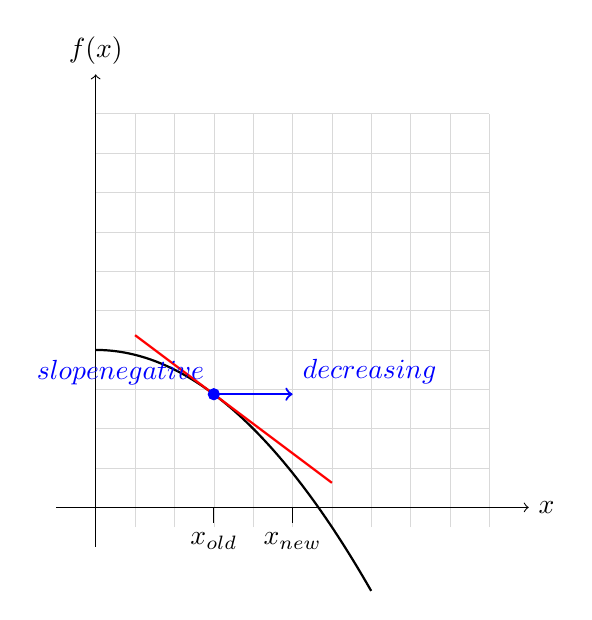
\begin{tikzpicture}[scale=1.0]
    % grid
    \draw[step=0.5, gray!30, very thin] (0,-0.25) grid (5,5);
    
    % axes
    \draw[->] (-0.5,0) -- (5.5,0) node[right] {$x$};
    \draw[->] (0,-0.5) -- (0,5.5) node[above] {$f(x)$};
    
    % function
    \draw[thick, domain=0:3.5, samples=100, smooth] plot (\x,{-0.25*\x*\x+2});
    
    % tangent line through x=1.5
    \draw[red, thick, domain=0.5:3] plot (\x,{-0.75*\x + 2.5625}); % tangent f'(1.5)=1.5
    
    % point on curve
    \filldraw[blue] (1.5,1.4375) circle (2pt) node[above left] {$\text{slope negative}$};
    
    % gradient descent arrow
    \draw[->, thick, blue] (1.5,1.4375) -- (2.5,1.4375) node[above right] {$\text{decreasing}$};
    
    % x labels
    \draw (1.5,0) -- (1.5,-0.2) node[below] {$x_\text{old}$};
    \draw (2.5,0) -- (2.5,-0.2) node[below] {$x_\text{new}$};
\end{tikzpicture}
\caption*{Slope $f'(x_\text{old})<0$: move right along $x$ to decrease $f(x)$.}
\end{minipage}
\end{figure}

\newpage
{\bf Gradient Descent Algorithm}\\

\enum{

\item Let's apply gradient descent to $f(x) = x^4 - 2x^2 + 1$ with $x_1 = 2$ and $\alpha = 0.02$. You will likely need technology (calculator, Desmos, etc.) to evaluate the derivative.

\enum{
\item Compute $f'(x)$.
\vs{1}
\item Evaluate $f'(x_1)$, and use this to compute a new guess $x_2$.
\tasksR{2}{
\task Find $\ds f^{\prime}(x_1).$ \vs{.25}
\task Find $\ds x_2$ using Gradient Descent algorithm. Round to $2$ decimal places. \vs{1.25}
}

\item Evaluate $f'(x_2)$, and use this to compute a new guess $x_3$.
\tasksR{2}{
\task Find $\ds f^{\prime}(x_2).$ Round to $2$ decimal places\vs{.25}
\task Find $\ds x_3$ using Gradient Descent algorithm. Round to $2$ decimal places. \vs{1.25}
}

\item Using our usual optimization tools (e.g. find critical numbers, decide if they are local max/min/neither, etc.), find the $x$-coordinate(s) of the local minima of $f(x)$.    Which minimum, if any, does $x_1$, $x_2$, $x_3, \dots$ seem to be approaching?
\vspace{4cm}
}
}

\newpage
\section*{Gradient Descent Exploration Activity}

Now open the Gradient Descent app found here: \href{https://woodword0-gradientdescentapplication.hf.space/}{Open the Gradient Descent App}\footnote{The direct link is \url{https://woodword0-gradientdescentapplication.hf.space/}}


\itemC{
    \item Select a function from the drop down menu
    \item Try different starting points $x_0$
    \item Try different learning rates $\alpha$ (both smaller and larger).
    \item Observe the sequence of points
}

\textbf{Answer the following questions:}

\begin{enumerate}

    \item For $f(x) = x^2$:
 \tasksI{2}{
        \task Does gradient descent always find the minimum?
       
        
        \task What happens if $\alpha$ is very large?
}
\vs{1}

    \item For $f(x) = e^x - x$:
 \tasksI{2}{
        \task Does the method converge to the same point from different starting values?
        \vspace{2cm}
        
        \task What do you notice about the slope near the minimum?
  }
\vs{1.5}

    \item For $f(x) = x^4 - 2x^2 + 1$:
\tasksI{2}{
        \task How many minimums does this function have?
    
        
        \task Does gradient descent always find the same minimum? How does the starting point affect the result?
    }

\end{enumerate}

\newpage
%%%%%%%%%%START HERE %%%%%%%%
\section*{During Class Application: Estimating Disease Spread with Gradient Descent}
In this activity. we will use gradient descent on real-world corona virus data to model a parameter called $R_0$ - the expected number of new infections produced by a single (typical/average) infectious individual.
The base reproduction number, $R_0$, (also called the base reproductive ratio) is defined as the expected number of new infections produced by a single (typical/average) infectious individual, when introduced into a totally susceptible population. $R_0$ is used in epidemiological studies of infectious diseases to gauge how contagious/transmissible an infectious disease is: if $R_0 < 1$, the disease will die out, and if $R_0 > 1$ infection can increase in the population. It is also used to determine how effective vaccination or other disease mitigation strategies need to be in order to protect populations from infection.
During the early stages of a disease outbreak, the number of cases often follows an exponential model:



\[
I(t) = e^{\lambda t}
\]
We can use this as a prediction function for the number of cases.
Taking the natural logarithm of both sides gives:
\[
\ln (I(t)) = \lambda t
\]

This transforms the exponential model into a \textbf{linear model}:
\[
\hat{y}(t) = \lambda t
\]
where:
\begin{itemize}
    \item $t$ = time (days),
    \item $\hat{y}(t) = \ln (I(t)) = \lambda t$ = predicted log of observed number of cases, and the prediction function.
    \item $\lambda$ = growth rate (how fast the infectious disease is spreading - unknown parameter).
\end{itemize}
\vspace{1cm}

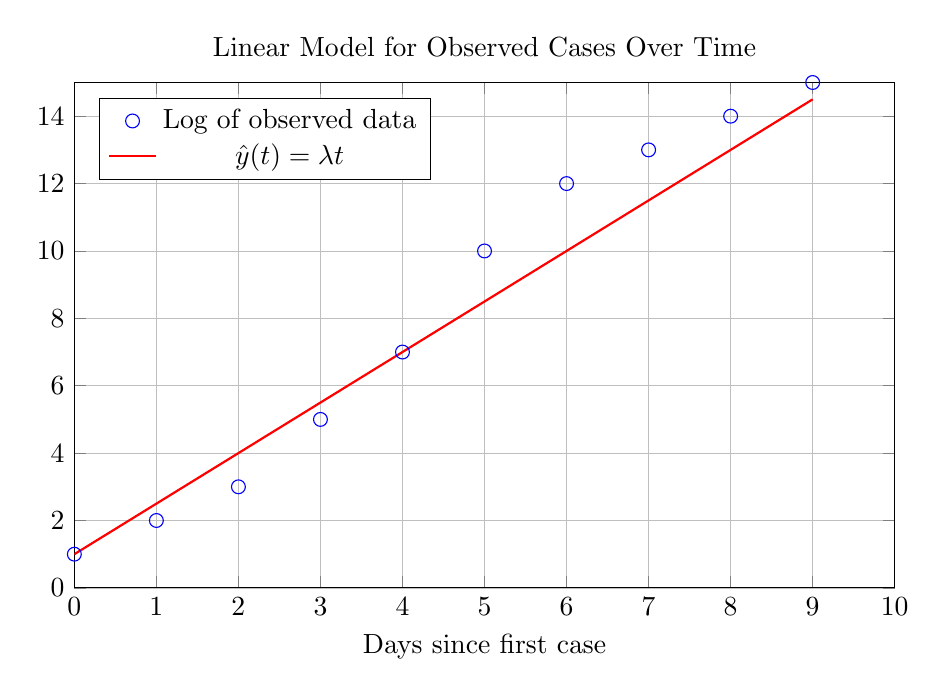
\begin{tikzpicture}
\begin{axis}[
    title={Linear Model for Observed Cases Over Time},
    xlabel={Days since first case},
  ylabel={},
  %$\log(\text{Number of Cases})$
    xmin=0, xmax=10,
    ymin=0, ymax=15,
    grid=both,
    major grid style={line width=.2pt,draw=gray!50},
    minor grid style={line width=.1pt,draw=gray!20},
    width=12cm,
    height=8cm,
    legend pos=north west,
]

% Data points
\addplot[
    only marks,
    mark=o,
    mark size=2.5pt,
    blue,
] coordinates {
    (0,1) (1,2) (2,3) (3,5) (4,7) (5,10) (6,12) (7,13) (8,14) (9,15)
};
\addlegendentry{Log of observed data}

% Line of best fit
\addplot[
    red,
    thick,
    domain=0:9,
] {1.5*x + 1};
\addlegendentry{$\hat{y}(t) = \lambda t$}

\end{axis}
\end{tikzpicture}

Our goal is to find the value of $\lambda$ that best fits the data.
\section*{Setting up Gradient Descent with a Single Data Point}
To start with, suppose we only have one data point $(t_0,y_0)$ of observed data.
%%%%%%%%%%%%%%%%%%%%%%%%%%%%%%%%%%%%%%%%%%%%%%%%%%%%%%%%%%%%%%%%%%%%%%%%%%%%%%%%%%%%%%%%%%%%%%%%%%%%%%%%%%%%%%%%%%%%%%%%%%%%%%%%%%%%%%%%%%%%%%%%%%%%%%%%%%%%%%%%%%%%%%%%%%%%%%%%%%%%%%%%%%%%%%%%%%%%%%%%%%%%%%%%%%%%%%%%%%%%
\begin{enumerate}

\item \textbf{Error Function with a Single data point}\\
%\textbf{The Initial Problem:} \\

We do not know the value of $\lambda$, but if we are given a single  data point consisting of two numbers $(t_1,\ln(I(t_1))) = (t_1,y_1)$,
we can use our gradient descent algorithm to try to find the value of $\lambda$ that makes our model match this data point. To do this we try to minimize the squared error between the data we have observed and our predictions:
\[
E(\lambda) = \big(y_1 - \lambda t_1\big)^2
\]
\item \textbf{Setting up gradient descent for a single data point.}\\
    We can now take the derivative with respect to our variable $\lambda$ of our error function $E(\lambda)$ using the chain rule.
  %      \begin{enumerate}
    To reduce the error, we:
    \begin{enumerate}
    \item[(a)] \textbf{Choose an initial guess} $\lambda_1 = \lambda_{\text{old}}$ for $\lambda$\\
    \item[(b)] \textbf{Compute a prediction} $\hat{y}_1(t_1) = \lambda_1 t_1$\\

    \item[(c)] \textbf{Compute the derivative} with respect to $\lambda$ of the error function:
    \[
    \frac{dE}{d \lambda} = 2\big(y_1 - \lambda t_1\big) \cdot (-t_1)
    \]
    \item[(d)] Then \textbf{update} $\lambda$ using:
    \al{
    \lambda_{\text{new}} &= \lambda_{\text{old}} - \alpha \cdot \frac{dE}{d\lambda} \\
      \lambda_{\text{new}}  &=\lambda_{\text{old}} - \alpha \cdot 2\big(y_1 + \lambda_{\text{old}}t_1\big)
   }
    where $\alpha > 0$ is the \textbf{step size} (learning rate).
    \end{enumerate}
    \vspace{0.5cm}
    
Overall, the process can be defined as follows:\\
\vspace{0.5cm}\

\textbf{Summary}
\begin{itemize}
    \item Choose an initial guess $\lambda_1$ for $\lambda$\\
    \item Compute your predictions.
    \item Compute the derivative of the error function.\\
    \item Update $\lambda$ with gradient descent.
\end{itemize}
\end{enumerate}
%%%%%%%%%%%%%%%%%%%%%%%%%%%%%%%%%%%%%%%%%%%%%%%%%%%%%%%%%%%%%%%%%%%%%%%%%%%%%%%%%%%%%%%%%%%%%%%%%%%%%%%%%%%%%%%%%%%%%%%%%%%%%%%%%%%%%%%%%%%%%%%%%%%%%%%%%%%%%%%%%%%%%%%%%%%%%%%%%%%%%%%%%%%%%%%%%%%%%%%%%%%%%%%%%%%%%%%%%%%%
\newpage
\subsection*{You Try!}

Suppose we observe the the spread of the disease for just one day and found the following data:

\[
\begin{array}{c|c}
t_i & y_i = \ln I(t_i) \\
\hline
1 & 1 \\
\end{array}
\]
So our single data point is $(t_1,y_1)=(1,1)$ Let's use this data point to update gradient descent algorithm manually for one step.\\\\
{\bf Choose an initial guess}:  \\ Let's assume
$\lambda_1 = 0.5, \quad \alpha = 0.1$\\
\\

\tasksA{2}{
\task {\bf Compute a prediction}:\\
$\ds 
\hat{y}_1 = \lambda_1 t_1 = 
$\\
\vspace{3cm}

% {\color{blue}
% \underline{$\hat{y}_1 = \lambda t_1  = 0.5\cdot (1) = 0.5$}
% }
\task  {\bf Compute derivative}:\\
\(\ds 
\frac{dE}{d\lambda} = 2(y_1 - \hat{y}_1)(-t_1) =
\)\\
\vs{2}

%{\color{blue}
%\begin{align*}
%    \frac{dE}{d\lambda} &= 2(y_1 - \hat{y}_1)(-t_1)\\
%    &= 2(1 - \lambda_1 t_1)(-t_1)\\
%    &= 2(1 - 0.5)(-1)\\
%    &= 2(0.5)(-1)\\
%    &= -1
%\end{align*}
%}
\task {\bf Update}:\\
$ \ds
\lambda_2 = \lambda_1 - \alpha \frac{dE}{d\lambda}
= 
$\\
\vspace{3cm}

% {\color{blue}
% \underline{$\lambda_2 = \lambda_1 - \alpha \frac{dE}{d\lambda} = 0.5 - (0.1) \cdot (-1) = 0.6$}
% }
}
%%%%%%%%%%%%%%%%%%%%%%%%%%%%%%%%%%%%%%%%%%%%%%%%%%%%%%%%%%%%%%%%%%%%%%%%%%%%%%%%%%%%%%%%%%%%%%%%%%%%%%%%%%%%%%%%%%%%%%%%%%%%%%%%%%%%%%%%%%%%%%%%%%%%%%%%%%%%%%%%%%%%%%%%%%%%%%%%%%%%%%%%%%%%%%%%%%%%%%%%%%%%%%%%%%%%%%%%%%%%
\newpage
\section*{Setting up Gradient Descent with several data points}
Now, suppose we have several data points $(t_1,y_1), (t_2,y_2) \ldots (t_{n},y_{n})$ of observed data.
It turns out that to get the error function we can just take an average over the squares of all of the errors; that is the differences between the observed values and the predicted values.
\vspace{1cm}

%\begin{center}
%
\includegraphics[width=0.6\linewidth]{Spring 2026/ApplicationDays/GradientDescent/images/MeanSquaredError.png}
%\end{center}

\begin{center}
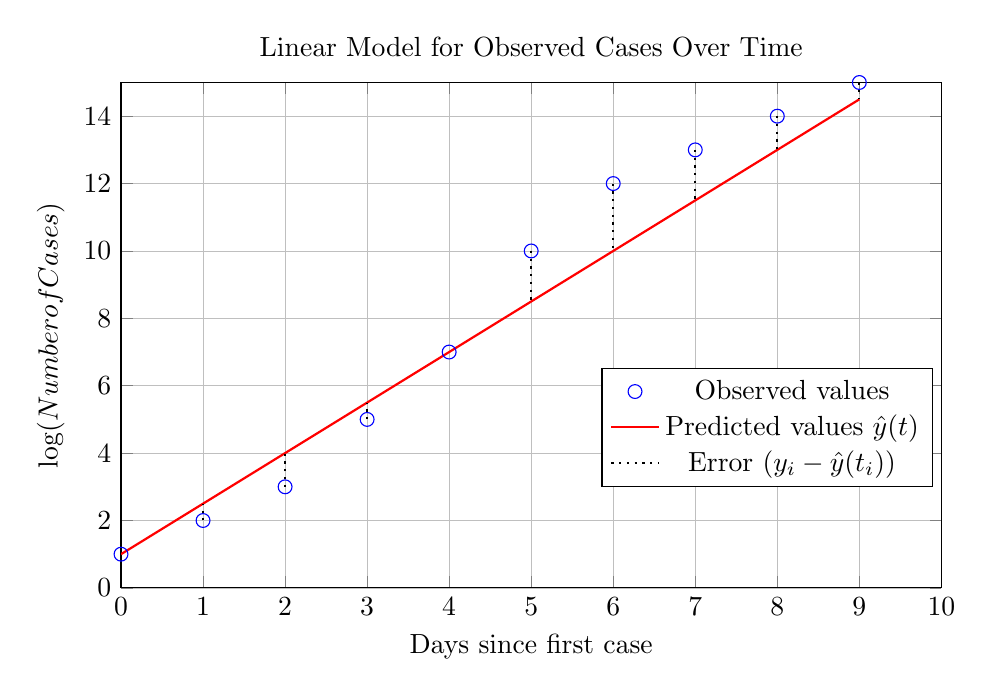
\begin{tikzpicture}
\begin{axis}[
    title={Linear Model for Observed Cases Over Time},
    xlabel={Days since first case},
    ylabel={$\log(\text{Number of Cases})$},
    xmin=0, xmax=10,
    ymin=0, ymax=15,
    grid=both,
    major grid style={line width=.2pt,draw=gray!50},
    minor grid style={line width=.1pt,draw=gray!20},
    width=12cm,
    height=8cm,
    legend style={
    at={(0.99,0.2)},
    anchor=south east
}
]

% Data points
\addplot[
    only marks,
    mark=o,
    mark size=2.5pt,
    blue,
] coordinates {
    (0,1) (1,2) (2,3) (3,5) (4,7) (5,10) (6,12) (7,13) (8,14) (9,15)
};
\addlegendentry{Observed values}

% Line of best fit
\addplot[
    red,
    thick,
    domain=0:9,
] {1.5*x + 1};
\addlegendentry{Predicted values $\hat{y}(t)$}

% Residual (error) lines
\addplot[
    black,
    dotted,
    thick,
    unbounded coords=jump,
] coordinates {
    (0,1) (0,1.5*0+1) (nan,nan)
    (1,2) (1,1.5*1+1) (nan,nan)
    (2,3) (2,1.5*2+1) (nan,nan)
    (3,5) (3,1.5*3+1) (nan,nan)
    (4,7) (4,1.5*4+1) (nan,nan)
    (5,10) (5,1.5*5+1) (nan,nan)
    (6,12) (6,1.5*6+1) (nan,nan)
    (7,13) (7,1.5*7+1) (nan,nan)
    (8,14) (8,1.5*8+1) (nan,nan)
    (9,15) (9,1.5*9+1)
};
\addlegendentry{Error $(y_i - \hat{y}(t_i))$}
\end{axis}
\end{tikzpicture}
\end{center}
\vspace{0.5cm}

\begin{enumerate}
\item \textbf{Error Function for several data points}

We measure how well our model fits the data by taking an average over all errors squared; that is the differences between the observed values and the predicted values. The error function becomes:
\[
E(\lambda) = \frac{1}{n} \sum_{i=1}^{n} \big(y_i - \lambda t_i \big)^2
\]
\item \textbf{Setting up Gradient Descent for several data points} \\
To reduce the error, we can use the same procedure as in the case of a single point:
    \begin{enumerate}
    \item[(a)] \textbf{Choose an initial guess} $\lambda_0 = \lambda_{\text{old}}$ for $\lambda$
    \item[(b)] \textbf{Compute predictions} $\hat{y}_i(t_i) = \lambda_1 t_i$\\

    \item[(c)] \textbf{Compute the derivative} of this error function using the chain rule and linearity properties of derivatives we learned in class:
    \[\frac{dE}{d\lambda} = \frac{1}{n} \sum_{i=1}^{n} 2(y_i - \lambda t_i)(-t_i)\]
    \item[(d)] Then \textbf{update} $\lambda$ using:
    \begin{align*}
    \lambda_{\text{new}} &= \lambda_{\text{old}} - \alpha \frac{dE}{d\lambda} \\
    &= \lambda_{\text{old}} - \alpha \cdot\frac{1}{n} \sum_{i=1}^{n} 2(y_i - \lambda_{\text{old}} t_i)(-t_i)\\
    \end{align*}
    where $\alpha > 0$ is the \textbf{step size} (learning rate).
    \end{enumerate}
\end{enumerate}
%%%%%%%%%%%%%%%%%%%%%%%%%%%%%%%%%%%%%%%%%%%%%%%%%%%%%%%%%%%%%%%%%%%%%%%%%%%%%%%%%%%%%%%%%%%%%%%%%%%%%%%%%%%%%%%%%%%%%%%%%%%%%%%%%%%%%%%%%%%%%%%%%%%%%%%%%%%%%%%%%%%%%%%%%%%%%%%%%%%%%%%%%%%%%%%%%%%%%%%%%%%%%%%%%%%%%%%%%%%%
%\newpage
\subsection*{You Try!}

Suppose we observe the the spread of the disease for just two days and found the following data:

\[
\begin{array}{c|c|c}
i&t_i & y_i = \ln \left(I(t_i)\right) \\
\hline
1&0 & 0 \\
2&1 & 0.7 \\
%2 & 1.4 \\
%3 & 2.1 \\
\end{array}
\]
So our data points are $(t_1,y_1)=(0,0)$ and $(t_2,y_2)=(1,0.7)$ Let's use these two data points to update gradient descent once.\\\\
{\bf Choose an initial guess}:  Let's assume
$
\lambda_1 = 0.5, \quad \alpha = 0.1
$\\

\begin{enumerate}


\item {\bf Compute predictions}:
\tasksR{2}{
\task $\hat{y}_1 = \lambda_1 t_1 = $\\
        % {\color{blue}
        % \underline{$\hat{y}_1 = \lambda_1 t_1  = 0.5(0) = 0$}
        % }
        \vspace{2cm}
        
        
   \task $\hat{y}_2 =
        $\\
        \vspace{2cm}
}
        
% {\color{blue}\underline{$\hat{y}_2 = \lambda_1 t_2 = 0.5(1) = 0.5$}
% }
\item {\bf   Compute derivative}:\\
$\ds 
\frac{dE}{d\lambda} = \frac{1}{2} \sum_{i=1}^2 2(y_i - \hat{y}_i)(-t_i)
= 
$\\
\vs{1.5}

% {\color{blue}
% \begin{align*}
%     \frac{dE}{d\lambda} &= -\frac{2}{4} \sum_{i=1}^2 (y_i - \hat{y}_i)t_i \\
%     &= -\frac{1}{2}\big((y_1 - \lambda t_1)t_1 + (y_2-  \lambda t_2)t_2\big)\\
%     &= -\frac{1}{2}\big((0 - 0)\cdot 0 + (0.7-  0.5)\cdot 1\big)\\
%     &= -\frac{1}{2}0.2\\
%     &= -0.1
% \end{align*}
% }
\item {\bf Update}:\\
$\ds 
\lambda_2 = \lambda_1 - \alpha \frac{dE}{d\lambda}
= 
$\\
\vspace{2cm}

% {\color{blue} 
% \begin{align*}
% \lambda_1 &= \lambda_0 - \alpha \frac{dE}{d\lambda} \\
% &= 0.5 - (0.1)\cdot (-0.1)\\
% &= 0.51
% \end{align*}
% }
\end{enumerate}
%\end{enumerate}
%\newpage
%%%%%%%%%%%%%%%%%%%%%%%%%%%%%%%%%%%%%%%%%%%%%%%%%%%%%%%%%%%%%%%%%%%%%%%%%%%%%%%%%%%%%%%%%%%%%%%%%%%%%%%%%%%%%%%%%%%%%%%%%%%%%%%%%%%%%%%%%%%%%%%%%%%%%%%%%%%%%%%%%%%%%%%%%%%%%%%%%%%%%%%%%%%%%%%%%%%%%%%%%%%%%%%%%%%%%%%%%%%%





\newpage





%%%%%%%%%%%%%%%%%%%%%%%%%%%%%%%%%%%%%%%%%%%%%%%%%%%%%%%%%%%%%%%%%%%%%%%%%%%%%%%%%%%%%%%%%%%%%%%%%%%%%%%%%%%%%%%%%%%%%%%%%%%%%%%%%%%%%%%%%%%%%%%%%%%%%%%%%%%%%%%%%%%%%%%%%%%%%%%%%%%%%%%%%%%%%%%%%%%%%%%%%%%%%%%%%%%%%%%%%%%%
\subsection*{Using Technology to Estimate Disease Spread}


We now use real-world data to estimate how quickly an infectious disease spreads.\footnote{Data source: Johns Hopkins University COVID-19 dataset, \texttt{https://github.com/CSSEGISandData/COVID-19}}
\medskip

\textbf{Goal:} Use gradient descent to estimate the exponential growth rate $\lambda$ from observed data.

\medskip

\textbf{Model Assumption (Early Outbreak):}

During the early stages of an outbreak, the number of cases grows approximately exponentially:
\[
I(t) \approx e^{\lambda t}
\]
\vspace{0.5cm}

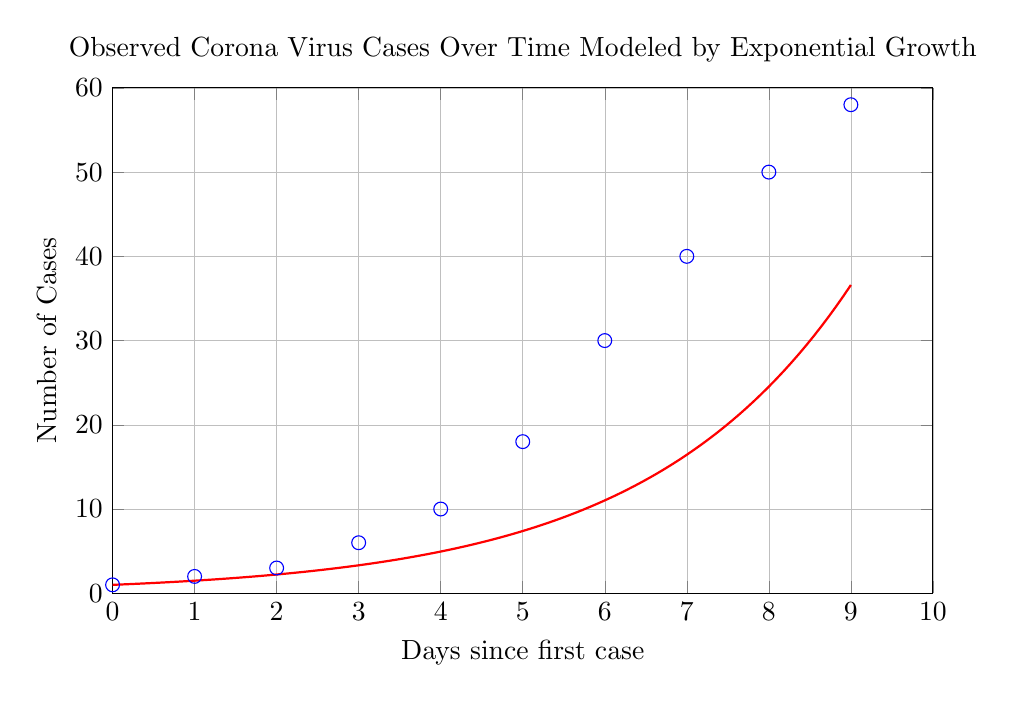
\begin{tikzpicture}
\begin{axis}[
    title={Observed Corona Virus Cases Over Time Modeled by Exponential Growth},
    xlabel={Days since first case},
    ylabel={Number of Cases},
    xmin=0, xmax=10,
    ymin=0, ymax=60,
    grid=both,
    major grid style={line width=.2pt,draw=gray!50},
    minor grid style={line width=.1pt,draw=gray!20},
    width=12cm,
    height=8cm,
    legend pos=north west,
]

% Example data points (roughly exponential)
\addplot[
    only marks,
    mark=o,
    mark size=2.5pt,
    blue,
] coordinates {
    (0,1) (1,2) (2,3) (3,6) (4,10) (5,18) (6,30) (7,40) (8,50) (9,58)
};
%\addlegendentry{Observed Data}

% Optional: line of best fit (exponential approximation using y = exp(0.4*x))
\addplot[
    red,
    thick,
    domain=0:9,
    samples=100,
] {exp(0.4*x)};
%\addlegendentry{Exponential Approximation}

\end{axis}
\end{tikzpicture}
\vspace{2cm}

Taking the natural logarithm gives a linear relationship:
\[
\ln(I(t)) \approx \lambda t
\]

\medskip


In this activity, we will:

\begin{enumerate}
    \item Run the gradient descent algorithm in an online application.
    \item Record the final estimated value of $\lambda$:
\end{enumerate}

\subsection*{Estimating $R_0$}

The base reproduction number $R_0$ measures how many people, on average, one infected person will infect.

It can be approximated using:
\[
R_0 \approx e^{\lambda T_g}
\]

where $T_g$ is the \textbf{mean generation time} (the average time between infections). For our covid dataset, $T_g \approx 3.5$ days

\medskip




\subsection*{Interpretation}

\begin{itemize}
    \item If $R_0 > 1$: the virus spreads exponentially.
    \item If $R_0 = 1$: the virus remains stable.
    \item If $R_0 < 1$: the virus dies out.
\end{itemize}

\medskip
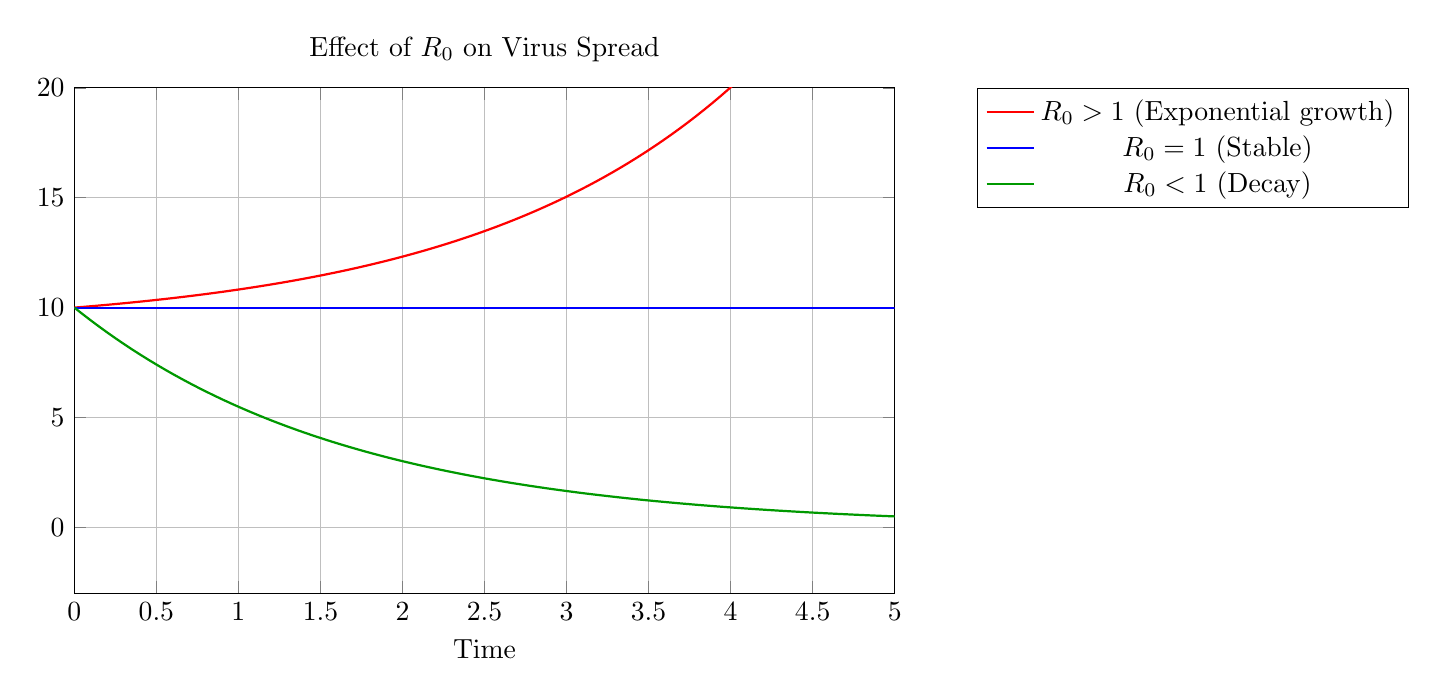
\begin{tikzpicture}
\begin{axis}[
    title={Effect of $R_0$ on Virus Spread},
    xlabel={Time},
    ylabel={},
    xmin=0, xmax=5,
    ymin=-3, ymax=20,
    grid=both,
    width=12cm,
    height=8cm,
    legend style={
        at={(1.1,1)},
        anchor=north west,
        fill=white,
        draw=black
    },
]

% R0 > 1 (growth)
\addplot[
    red,
    thick,
    domain=0:5,
    samples=100,
] {exp(0.6*x) + 9};
\addlegendentry{$R_0 > 1$ (Exponential growth)}

% R0 = 1 (constant)
\addplot[
    blue,
    thick,
    domain=0:5,
] {10};
\addlegendentry{$R_0 = 1$ (Stable)}

% R0 < 1 (decay)
\addplot[
    green!60!black,
    thick,
    domain=0:5,
    samples=100,
] {10*exp(-0.6*x)};
\addlegendentry{$R_0 < 1$ (Decay)}

\end{axis}
\end{tikzpicture}
% \begin{figure}[h!]
%     \centering
%     
\includegraphics[width=0.4\linewidth]{Spring 2026/ApplicationDays/GradientDescent/images/R_0Graph.png}
%     \caption{$R_0$ measures how many people, on average, one infected person will infect.}
%     \label{fig:R0Graph}
% \end{figure}
\vspace{0.5cm}



%\newpage
Use this link \href{https://woodword0-gradientdescentapplication2.hf.space/}{Open the Gradient Descent App}\footnote{The direct link i \url{https://woodword0-gradientdescentapplication2.hf.space/}} to answer the following questions:
\begin{enumerate}
\item First start with any fixed guess for $\lambda$, $\alpha$ and the number of steps. You can see how well the line $\lambda t$ approximates the dataset in the first graph ``Initial Model vs Data." Click the ``Run Gradient Descent" button to get an estimate for the true value of $\lambda$. 
\tasksA{2}{
   \task What value do you get for $\lambda$? 
    \vspace{3cm}
    
    \task What is the error of your estimate?
    \vspace{3cm}

  \task Click the ``Compute $R0$" button. What value did you get for $R_0$?
    \vspace{3cm}

    \task What does this value for $R0$ tell us in the context of this problem?
    \vspace{3cm}


}
\newpage

\item Now lets try to tune the parameters of the model.
\tasksA{2}{
\task  Now keep $\alpha$ the same as before but change the number of steps to $50$.  What is the new value for $\lambda$? For Error? How does changing the number of steps affect the error?


\task Now keep the number of steps as in part $1$ of this exploration  and change $\alpha$ to 0.01. How does changing the learning rate affect the error?
\vs{3}

\task* Experiment with different values  for $\alpha$ and the Number of steps try to get the smallest error you can using the least number of steps possible.  What values do you get for $\lambda$? For Error? Which values for $\alpha$ and Number of steps did you use to get these values?




}
\vspace{4cm}



\newpage

\item  Now change the Initial guess for $\lambda$ to further tune your parameters for $\alpha$ and Number of steps to get the smallest error you can using the least amount of steps. 
   \tasksA{2}{
    \task What initial value did you choose for  $\lambda$? For $\alpha$?
   \vs{2}
    
  \task  What value do you get for the approximated $\lambda$? 
  
    
\task How many steps did your model need to converge to the minimal error?
\vs{2}
    
   \task  What value do you get for $R_0$? This represents the number of people that one person will infect (on average).
    \vspace{3cm}
    
    \task What is the error of your estimate?
    \vspace{3cm}

}




    
\newpage
\item An epidemiologist at the National Institutes of Health is preparing a grant proposal to request emergency funding in response to a viral outbreak. Rather than making a simple yes/no recommendation, they must estimate how much funding will be needed based on projected disease spread.


Assume:
\itemI{
    \item Each infected individual costs the healthcare system \$10{,}000 on average.
    \item Each \$100{,}000 of preventative measures (funded by the grant) can reduce the effective reproduction number by 5\%.
}


\begin{enumerate}
    \item[(a)]  Using your estimated value of $R_0$, project the average number people that 1{,}000 people will infect.
        \vspace{3cm}
%{\color{blue}
%$1000 \times R_0 = a$ cases.
%}
    \item[(b)]  Estimate the average number people that 1{,}000 people will infect if the grant is funded and $R_0$ is reduced by 5\%.
        \vspace{3cm}
%{\color{blue}
%$R_0*(1 - 0.05)(1{,}000) = b$ cases.
%}
    \item[(c)]  If each infected individual costs the healthcare system \$10{,}000 on average, calculate the total cost savings  for 1{,}000 people due to intervention.
        \vspace{3cm}
%{\color{blue}
%$a - b = \$$.
%}
    \item[(d)] How much funding would be required to stabilize the virus?
        \vspace{3cm}
%{\color{blue}
% $R_0(1 - 0.05)^n = 1 \implies (0.95)^n = \frac{1}{R_0} \implies n = \frac{-\ln(R_0)}{(0.95)}$.
% Funding Required = n \times 100{,}000.
%}   

\end{enumerate}

\end{enumerate}


\end{document}  
